% Options for packages loaded elsewhere
\PassOptionsToPackage{unicode}{hyperref}
\PassOptionsToPackage{hyphens}{url}
%
\documentclass[
]{book}
\usepackage{amsmath,amssymb}
\usepackage{iftex}
\ifPDFTeX
  \usepackage[T1]{fontenc}
  \usepackage[utf8]{inputenc}
  \usepackage{textcomp} % provide euro and other symbols
\else % if luatex or xetex
  \usepackage{unicode-math} % this also loads fontspec
  \defaultfontfeatures{Scale=MatchLowercase}
  \defaultfontfeatures[\rmfamily]{Ligatures=TeX,Scale=1}
\fi
\usepackage{lmodern}
\ifPDFTeX\else
  % xetex/luatex font selection
\fi
% Use upquote if available, for straight quotes in verbatim environments
\IfFileExists{upquote.sty}{\usepackage{upquote}}{}
\IfFileExists{microtype.sty}{% use microtype if available
  \usepackage[]{microtype}
  \UseMicrotypeSet[protrusion]{basicmath} % disable protrusion for tt fonts
}{}
\makeatletter
\@ifundefined{KOMAClassName}{% if non-KOMA class
  \IfFileExists{parskip.sty}{%
    \usepackage{parskip}
  }{% else
    \setlength{\parindent}{0pt}
    \setlength{\parskip}{6pt plus 2pt minus 1pt}}
}{% if KOMA class
  \KOMAoptions{parskip=half}}
\makeatother
\usepackage{xcolor}
\usepackage{graphicx}
\makeatletter
\def\maxwidth{\ifdim\Gin@nat@width>\linewidth\linewidth\else\Gin@nat@width\fi}
\def\maxheight{\ifdim\Gin@nat@height>\textheight\textheight\else\Gin@nat@height\fi}
\makeatother
% Scale images if necessary, so that they will not overflow the page
% margins by default, and it is still possible to overwrite the defaults
% using explicit options in \includegraphics[width, height, ...]{}
\setkeys{Gin}{width=\maxwidth,height=\maxheight,keepaspectratio}
% Set default figure placement to htbp
\makeatletter
\def\fps@figure{htbp}
\makeatother
\setlength{\emergencystretch}{3em} % prevent overfull lines
\providecommand{\tightlist}{%
  \setlength{\itemsep}{0pt}\setlength{\parskip}{0pt}}
\setcounter{secnumdepth}{-\maxdimen} % remove section numbering
\ifLuaTeX
  \usepackage{selnolig}  % disable illegal ligatures
\fi
\usepackage{bookmark}
\IfFileExists{xurl.sty}{\usepackage{xurl}}{} % add URL line breaks if available
\urlstyle{same}
\hypersetup{
  pdftitle={mtbook\_uebungen},
  hidelinks,
  pdfcreator={LaTeX via pandoc}}

\title{mtbook\_uebungen}
\author{}
\date{Dez 24, 2022}

\begin{document}
\frontmatter
\maketitle

\mainmatter
\section{Abtastung eines Dreiecksignals}\label{abtastung-eines-dreiecksignals}

Ein als ideal angenommenes Dreiecksignal mit einer Periodendauer von \(1\,\mathrm{ms}\) werde mit einer Abtastrate von \(10\,\mathrm{kHz}\) digitalisiert. Geben Sie an, ob in diesem Fall das Abtasttheorem nach Shannon erfüllt ist! Begründen Sie Ihre Antwort!

Welcher Effekt tritt ein, wenn das Abtasttheorem verletzt ist? Erläutern Sie diesen Effekt mit einer einfachen Skizze.

\section{Aliasing bei der Digitalisierung von Musik}\label{aliasing-bei-der-digitalisierung-von-musik}

Sie planen, ein Musiksignal zu digitalisieren und hierfür einen A/D-Umsetzer mit einer Abtastfrequenz von \(44,1\,\mathrm{kHz}\) zu verwenden. Sie wissen, dass in dem analogen Musiksignal Frequenzanteile bis hinauf zu \(50\,\mathrm{kHz}\) enthalten sind, deren Amplitude nicht vernachlässigbar ist. Ihnen ist bewusst, dass für diese hohen Frequenzanteile das Abtasttheorem nach Shannon verletzt wird. Ihr Kommilitone schlägt vor, die A/D- Umsetzung dennoch wie geplant vorzunehmen und argumentiert, dass Frequenzen von über \(20\,\mathrm{kHz}\) für den Menschen ohnehin nicht hörbar seien und es daher keine Rolle spiele, wenn diese nicht korrekt digitalisiert werden.

Geben Sie an, ob Sie dieser Argumentation folgen würden oder nicht! Begründen Sie Ihre Antwort!

\section{Bestimmung des Drehmomentes einer Welle}\label{bestimmung-des-drehmomentes-einer-welle}

Das Drehmoment einer Welle wird mit Hilfe der DMS-Messtechnik gemessen. Dehnungsmessstreifen (DMS) ändern aufgrund einer relativen Längenänderung \(\epsilon = \frac{\Delta L}{L}\) ihren Widerstandswert \(R(\epsilon) = k\epsilon\). Der \(k\)-Faktor beträgt hier 2,01 und der Widerstand beträgt \(300\,\Omega\). DMS messen entlang einer Achse Längenänderung.

\begin{figure}
\centering
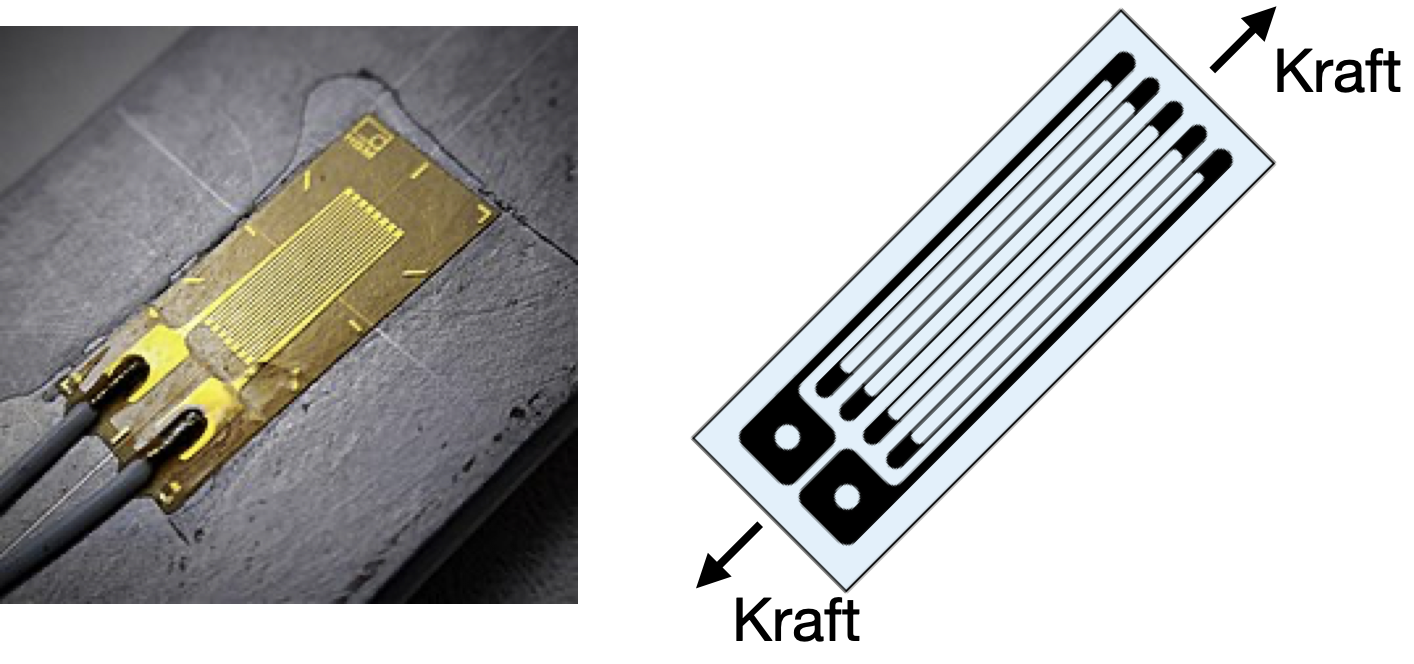
\includegraphics{pictures/DMS.png}
\caption{Dehnungsmesstreifen (DMS)}
\end{figure}

In dieser Aufgaben sollen DMS benutzt werden, um das Drehmoment einer Welle zu bestimmen. Sie können entsprechend der Skizze die DMS unter einem Winkel von 45 Grad zur Längsachse der Welle anbringen. Die DMS der +45 Grad-Linie werden dadurch um \(+\epsilon\) gedehnt und die der -45 Grad-Linie werden betragsmäßig gleich groß um \(-\epsilon\) gestaucht.

\begin{figure}
\centering
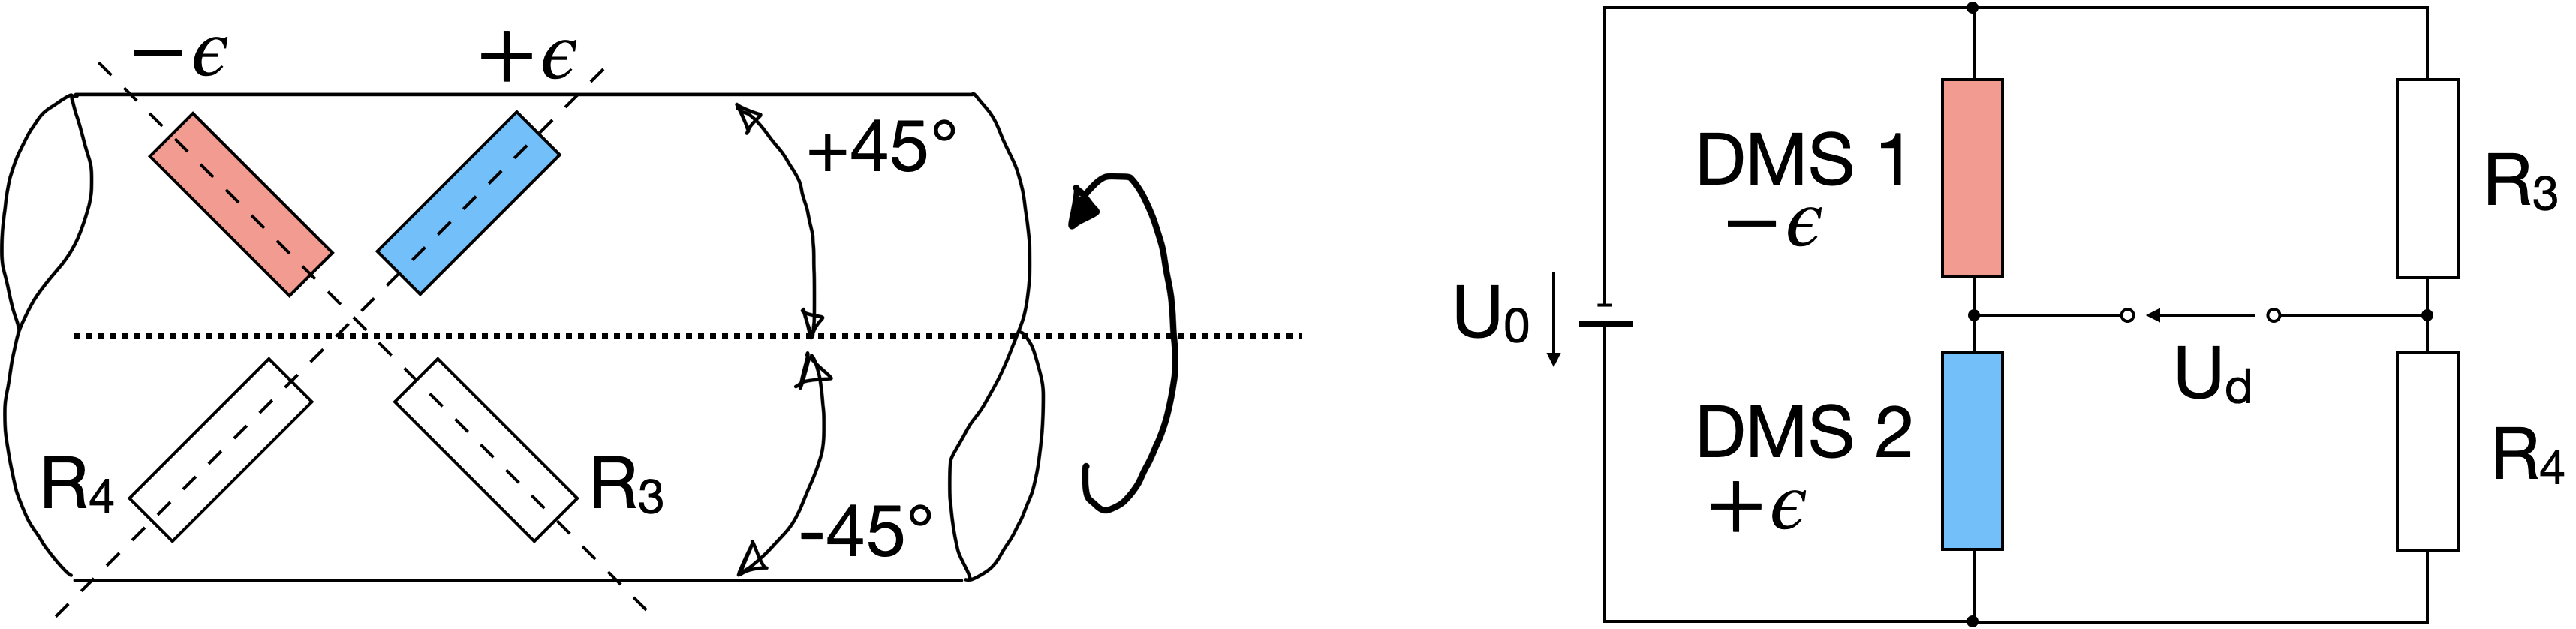
\includegraphics{pictures/DMS_messbruecke.png}
\caption{Links: Anordnung der DMS auf der Welle an 45 Grad-Linie. Rechts: Anordnung der DMS in der Messbrücke}
\end{figure}

Die Welle hat einen Durchmesser \(D = 3{,}1\,\mathrm{cm}\), einen Elastizitätsmodul \(E = 20{,}5 \cdot 10^{4}\,\mathrm{N/mm^{2}}\) und eine Querdehnungszahl von \(\mu = 0{,}31\). Es wird eine Wheatstonesche Messbrücke mit Gleichstromspeisung verwendet, die im Ausschlagverfahren arbeitet und mit einer Gleichspannung von \(U = 3{,}5\,\mathrm V\) versorgt wird. Zwischen Drehmoment \(M_{D}\) und Dehnung \(\varepsilon\) besteht folgende Beziehung:

\[M_{D} = \frac{E \pi D^{3} \epsilon}{16 (1+\mu)}\]

Die Formel für die Diagonalspannung \(U_{d}\) in Abhängigkeit von \(\epsilon\) ist:

\[U_{d} = \frac{1}{2}U_{0}k \epsilon\]

\begin{enumerate}
\def\labelenumi{\arabic{enumi}.}
\tightlist
\item
  Die Brücke soll abgeglichen sein, wenn kein Drehmoment angreift. Wie groß sind die übrigen beiden Widerstände der Messbrücke?
\end{enumerate}

```\{tip\} :class: dropdown Für den Abgleich gilt \(U_d = 0\) und somit

\[\frac{R_1}{R_2} = \frac{R_3}{R_4}\]

\begin{verbatim}

2. Ist die von Ihnen gewählte Messbrücke temperaturkompensiert?

```{tip}
:class: dropdown
Vergleichen Sie hierfür die Anschaltung der DMS mit der Aufgabe [Ausschlagsmessbrücke]{Aussschlag-Messbrücke.md}.
\end{verbatim}

\begin{enumerate}
\def\labelenumi{\arabic{enumi}.}
\setcounter{enumi}{2}
\tightlist
\item
  Wie groß ist der in einem der beiden DMS fließende Strom?
\end{enumerate}

```\{tip\} :class: dropdown Benutzen Sie ohm'sches Gesetz und betrachten Sie die Masche ganz linka:

\[U_ 0 = RI\]

Wie berechnet sich \(R\), bestehend aus einer Reihenschaltung der beiden DMS?

\begin{verbatim}

4. Wie groß ist das Drehmoment, wenn eine Brückenausgangsspannung von $880\,\mathrm{\mu V}$ angezeigt wird?

```{tip}
:class: dropdown
Formen Sie die Gleichung $U_{d} = \frac{1}{2}U_{0}k \epsilon$ nach $\epsilon$ um und setzen sie die in die Gleichung für $M_D$ ein. Setzen Sie alle Werte ein. ($M_D = 229\,\mathrm{Nm}$)
\end{verbatim}

\begin{enumerate}
\def\labelenumi{\arabic{enumi}.}
\setcounter{enumi}{4}
\tightlist
\item
  Welcher relative Maximal-Fehler ergibt sich für das unter d) ermittelte Drehmoment, wenn der Wellendurchmesser einen Fehler von \(\pm 0,2\,\mathrm{mm}\) aufweist und die Brückenspeisespannung auf \(\pm 3\)\% stabilisiert ist? Die übrigen Elemente der Messbrücke seien fehlerfrei.
\end{enumerate}

```\{tip\} :class: dropdown Für den absoluten Maximalfehler gilt:

\[\Delta y = \left| \frac{\partial y}{\partial x_1} \right| \cdot \Delta x_1+ \left|\frac{\partial y}{\partial x_2} \right| \cdot \Delta x_2 + \cdots\]

Spezialfall: Bei Multiplkation/Division addieren sich die \emph{relativen} Messabweichungen und es folgt für den relativen Fehler:

\[\pm \frac{\Delta M_D}{M_D} = 3 \cdot \frac{\Delta D}{D} + \frac{\Delta U_0}{U_0} = 4{,}935\%\]

\begin{verbatim}

6. Wie groß ist der absolute Maximal-Fehler?

```{tip}
:class: dropdown

$$ \Delta M_D = 11{,}3\,\mathrm{Nm}$$
\end{verbatim}

\section{Bode-Diagramm}\label{bode-diagramm}

Zur Darstellung von Übertragungsverhalten werden Bode-Diagramme zur Darstellung des Frequenzgangs benutzt. Durch die logarithmische Darstellung der Amplitudenverhältnisse lassen sich aus mehreren Übertragungssystemen zusammengesetzte Systeme leichter analysieren. Die logarithmische Darstellung bildet nämlich die Multiplikation der einzelnen Funktionen auf eine einfache Addition ab.

Es sei folgendes Übertragungssystem gegeben:

```\{figure\} pictures/bode.png :class: .dark-light --- height: 150px name: optional-label --- Übertragungssystem mit vier Gliedern.

\begin{verbatim}


welches aus einem P-Glied, einem D-Glied, einem PT1-Glied und einen PD-Glied besteht. 

$$H_1 = 10$$

$$H_2 = s$$

$$H_3 = \frac{1}{1+\frac{s}{4}}$$

$$H_4 = 1+\frac{s}{60}$$

Erstellen Sie das Bode-Diagramm, indem Sie die Amplitudengänge in dB eintragen und anschließend grafisch addieren. Analog erstellen Sie das Phasengang-Diagramm. 

![png](pictures/bode_blanko.png)


````{tip}
:class: dropdown
Was gilt für die Hintereinanderschaltung von Messsystemen im Laplace, bzw. Frequenzbereich? Schreiben Sie die Gesamt-Übertragungsfunktion hin.

<iframe width="560" height="315" src="https://www.youtube.com/embed/cQH--8rpRw8?si=uPyVg9Jesb0BtUJU" title="YouTube video player" frameborder="0" allow="accelerometer; autoplay; clipboard-write; encrypted-media; gyroscope; picture-in-picture; web-share" allowfullscreen></iframe>
\end{verbatim}

\section{Aliasing bei der Digitalisierung von Musik}\label{aliasing-bei-der-digitalisierung-von-musik-1}

Sie planen, ein Musiksignal zu digitalisieren und hierfür einen A/D-Umsetzer mit einer Abtastfrequenz von \(44,1\,\mathrm{kHz}\) zu verwenden. Sie wissen, dass in dem analogen Musiksignal Frequenzanteile bis hinauf zu \(50\,\mathrm{kHz}\) enthalten sind, deren Amplitude nicht vernachlässigbar ist. Ihnen ist bewusst, dass für diese hohen Frequenzanteile das Abtasttheorem nach Shannon verletzt wird. Ihr Kommilitone schlägt vor, die A/D- Umsetzung dennoch wie geplant vorzunehmen und argumentiert, dass Frequenzen von über \(20\,\mathrm{kHz}\) für den Menschen ohnehin nicht hörbar seien und es daher keine Rolle spiele, wenn diese nicht korrekt digitalisiert werden.

Geben Sie an, ob Sie dieser Argumentation folgen würden oder nicht! Begründen Sie Ihre Antwort!

\section{Abtastung eines Dreiecksignals}\label{abtastung-eines-dreiecksignals-1}

Ein als ideal angenommenes Dreiecksignal mit einer Periodendauer von \(1\,\mathrm{ms}\) werde mit einer Abtastrate von \(10\,\mathrm{kHz}\) digitalisiert. Geben Sie an, ob in diesem Fall das Abtasttheorem nach Shannon erfüllt ist! Begründen Sie Ihre Antwort!

Welcher Effekt tritt ein, wenn das Abtasttheorem verletzt ist? Erläutern Sie diesen Effekt mit einer einfachen Skizze.

\section{Aussschlagsmessbrücke}\label{aussschlagsmessbruxfccke}

Gegeben ist eine Ausschlagmessbrücke bestehend aus den beiden Spannungsteilern \(R_1\) und \(R_2\), bzw. \(R_3\) und \(R_4\).

\texttt{\{figure\}\ pictures/MB\_1.png\ :class:\ .dark-light\ -\/-\/-\ height:\ 150px\ -\/-\/-\ Messbrücke}

\subsection{Aufgabe 1: Diagonalspannung}\label{aufgabe-1-diagonalspannung}

Berechnen Sie die Diagonalspannung \(U_d\) einer Ausschlag-Messbrücke.

\texttt{\{tip\}\ :class:\ dropdown\ *\ Schreiben\ Sie\ die\ beiden\ Spannungsteiler-Gleichungen\ auf\ *\ Subtrahieren\ Sie\ die\ beiden\ Spannungswerte,\ z.B.\ \$U\_d\ =\ U\_2-U\_4\$}

\subsection{Aufgabe 2: Sensor}\label{aufgabe-2-sensor}

Mit der Brücke soll die Widerstandsänderung \(\Delta R\) eines Sensors, gegeben durch \(R_2 = R_x = R_0 + \Delta R + \Delta R_T\) (Temperaturfehler \(\Delta R_T\)) erfasst werden. Die anderen Brückenwiderstände sind mit \(R_0\) anzunehmen.

\begin{itemize}
\tightlist
\item
  Skizzieren Sie die Schaltung
\item
  Berechnen Sie \(U_d = f(U_0, \Delta R, \Delta R_T, R_0)\).
\end{itemize}

\texttt{\{tip\}\ :class:\ dropdown\ *\ Ersetzen\ Sie\ \$R\_2\$\ in\ der\ Gleichung\ von\ Aufgabe\ 1,\ sowie\ alle\ anderen\ Widerstände\ durch\ \$R\_0\$\ und\ vereinfachen\ Sie\ die\ Gleichung\ für\ \$U\_d\$.}

\subsection{Aufgabe 3: Temperaturkompensation}\label{aufgabe-3-temperaturkompensation}

Die Temperaturabhängigkeit \(\Delta R_T\) soll verringert werden. Hierzu steht Ihnen ein Widerstand mit identischem Temperaturverhalten zur Verfügung: \(R_K = R_0 + \Delta R_T\). Zeigen Sie, dass mit Hilfe von \(R_K\) der Einfluss von \(\Delta R_T\) stark reduziert werden kann. Gehen Sie folgendermaßen vor:

\begin{itemize}
\tightlist
\item
  Geben Sie eine geeignete Brückenschaltung an.
\item
  Berechnen Sie \(U_d = f(U_0, \Delta R, \Delta R_T, R_0)\).(Zwischenergebnisse sind im nächsten Punkt angegeben.)
\item
  Berechnen Sie die Empfindlichkeit in Abhängigkeit von \(\Delta R_T\) für die beiden Fälle mit und ohne \(R_K\).
\end{itemize}

\[E_{1}  = \frac{dU_d}{d\Delta R_T} \quad \textrm{mit} \quad U_d = \frac{U_0}{2} \cdot \frac{\Delta R + \Delta R_T}{2R_0 + \Delta R + \Delta R_T} \quad \textrm{ohne} \quad R_{K}\] \[E_2 = \frac{dU_d}{d\Delta R_T} \quad \textrm{mit} \quad U_d = \frac{U_0}{2} \cdot \frac{\Delta R}{2R_0 + \Delta R + 2\Delta R_T} \quad \textrm{mit} \quad R_{K}\]

\begin{itemize}
\tightlist
\item
  Bilden Sie den Quotienten aus beiden Resultaten, \(\frac{E_{1}}{E_{2}}\) und nähern Sie für \(\Delta R_{T} << R_{0}\).
\end{itemize}

\texttt{\{tip\}\ :class:\ dropdown\ *\ Setzen\ Sie\ \$R\_K\$\ an\ die\ Stelle\ von\ \$R\_1\$,\ also\ in\ den\ gleichen\ Spannungsteiler.\ *\ Die\ Empfindlichkeit\ berechnen\ Sie\ über\ die\ Ableitung,\ hier\ die\ Ableitung\ nach\ \$d\ \textbackslash{}Delta\ R\_T\$,\ wenn\ Sie\ die\ Empfindlichkeit\ für\ \$\textbackslash{}Delta\ R\_T\$\ haben\ möchten.}

\begin{itemize}
\tightlist
\item
  Setzen Sie Beispielwerte ein:
\end{itemize}

\[R_0 = 1\,\mathrm{k\Omega}\]

\[\Delta R = 100\,\mathrm\Omega\]

\[\Delta R_T = 0-1000\,\mathrm\Omega\]

\[U_0 = 10\,\mathrm V\]

```\{admonition\} Kontrollergebnisse :class: dropdown * Diagonalspannung allgemein:

\[\frac{U_d}{U_0} = U_2 - U_4 = \frac{R_2}{R_1+R_2} - \frac{R_4}{R_3+R_4}\]

\begin{itemize}
\tightlist
\item
  Diagonalspannung mit Sensor bei \(R_2 = R_x = R_0 + \Delta R + \Delta R_T\) und Empfindlichkeit E\_1\$:
\end{itemize}

\[U_d = \frac{U_0}{2} \cdot \frac{\Delta R + \Delta R_T}{2R_0 + \Delta R + \Delta R_T}\]

\[E_1 = \frac{dU_d}{d\Delta R_T} = \frac{U_0}{2} \frac{2R_0}{(2R_0 + \Delta R + \Delta R_T)^2}\]

\begin{itemize}
\tightlist
\item
  Diagonalspannung mit Sensor bei \(R_2 = R_x = R_0 + \Delta R + \Delta R_T\) und Korrekturwiderstand gegen Temperaturänderungen, \(R_1 = R_K\) und Empfindlichkeit \(E_2\):
\end{itemize}

\[U_d = \frac{U_0}{2} \cdot \frac{\Delta R}{2R_0 + \Delta R + 2\Delta R_T}\]

\[  = \frac{U_0}{2} \frac{-2\Delta R}{(2R_0 + \Delta R + \Delta 2R_T)^2}\]

\begin{itemize}
\tightlist
\item
  Verhältnis: Wir nehmen an, dass der Fehler aufgrund von Temperatur, \(\Delta R_T\), klein im Vergleich zum Widerstandswert \(R_0\) ist, sodass \(2 \Delta R_T \approx \Delta R_T\). Dadurch kürzt sich der Nenner weg, wenn die beiden Empfindlichkeiten ins Verhältnis gesetzt werden und es folgt:
\end{itemize}

\[r \approx -\frac{R_0}{\Delta R} = \frac{10000}{100} = 100\]

Die Möglichkeit Temperatur zu unterdrücken wird hauptsächlich durch die Wahl von den nominellen Widerstandswerten \(R_0\) bestimmt, die in der Brücke verbaut sind, und der zu messenden Größe \(\Delta R\). Je größer der Abstand zwischen \(R_0\) und \(\Delta R\), desto besser ist die Rauschunterdrückung. ```

\section{Empfindlichkeit eines Messgerätes}\label{empfindlichkeit-eines-messgeruxe4tes}

Geben Sie an, welche der folgenden Aussagen hinsichtlich der Empfindlichkeit eines Messgerätes zutreffend sind!

\begin{itemize}
\tightlist
\item
  Die Empfindlichkeit eines Messgerätes ist definiert als Steigung der Kennlinie im jeweiligen Arbeitspunkt.
\item
  Der k-Faktor bzw. die Dehnungsempfindlichkeit beim Dehnungsmessstreifen ist materialunabhängig.
\item
  Die Linearitätsabweichung von Kennlinien kann in Kalibrier- und Eichlaboren bestimmt werden.
\item
  Um die Gesamtempfindlichkeit zu ermitteln, werden die Empfindlichkeiten der einzelnen Glieder einer Messkette aneinander addiert.
\item
  Durch Herabsetzen des Messbereiches können Nichtlinearitäten in der Kennlinie vermieden werden.
\end{itemize}

\section{Digitalisierung}\label{digitalisierung}

Ein analoges Spannungssignal im Bereich von \(-12\,\mathrm V\) bis \(+12\,\mathrm V\) soll so digitalisiert werden, dass der maximale Quantisierungsfehler \(2\,\mathrm{mV}\) beträgt. Geben Sie an, mit wie viel Bit der A/D-Umsetzer mindestens arbeiten muss!

\begin{itemize}
\tightlist
\item
  \(11\) Bit
\item
  \(12\) Bit
\item
  \(13\) Bit
\item
  \(14\) Bit
\item
  \(15\) Bit
\item
  \(16\) Bit
\end{itemize}

\backmatter
\end{document}
